\documentclass[12pt]{ecsproject}     % Use the Project Style

\let\cleardoublepage\clearpage %eliminate blank pages between chapters

\usepackage{color}
\usepackage{graphicx}
\usepackage{lscape}
\usepackage{paralist}
\usepackage{url}
\usepackage{listings}
\usepackage{natbib}            % Use Natbib style for the refs.
\usepackage[nottoc]{tocbibind} %this will add bibliography to toc

%various configs
\graphicspath{{./figures/}}

\bibliographystyle{plainnat}

\definecolor{purple}{RGB}{153,0,153}
\definecolor{yellow}{RGB}{255,255,0}
\definecolor{blue}{RGB}{0,255,255}

\hypersetup{colorlinks=false}   % Set to false for black/white printing
%end configs

%% ----------------------------------------------------------------
%% Definitions.tex
%% ---------------------------------------------------------------- 
\newcommand{\BibTeX}{{\rm B\kern-.05em{\sc i\kern-.025em b}\kern-.08em T\kern-.1667em\lower.7ex\hbox{E}\kern-.125emX}}

%% People
\newcounter{address}
\setcounter{address}{1}
\renewcommand{\theaddress}{\textsuperscript{\fnsymbol{address}}}
\newcommand{\address}[1]{\refstepcounter{address}\theaddress#1\\}
\newcommand{\Name}[3]{\texorpdfstring{\href{mailto:#3}{#2}#1}{#2}\xspace}
\newcommand{\SteveRGunn}[1]{\Name{#1}{Steve R. Gunn}{S.R.Gunn@ecs.soton.ac.uk}}

%% Dingbats
\newcommand{\tick}{\ding{51}}
\newcommand{\cross}{\ding{55}}

%% Calculus
\newcommand{\pd}[2]{\ensuremath{\frac{\partial #1}{\partial #2}}\xspace}
\newcommand{\fd}[2]{\ensuremath{\frac{d #1}{d #2}}\xspace}
\newcommand{\dint}{\ensuremath{\int\!\!\!\int}\xspace}
\newcommand{\tint}{\ensuremath{\int\!\!\!\int\!\!\!\int}\xspace}

%% Math Sets
\newcommand{\Q}[1]{\ensuremath{\mathbb{#1}}\xspace}
\newcommand{\R}{\Q{R}}

%% Matrix, Vector
\newcommand{\V}[1]{\ensuremath{\boldsymbol{#1}}\xspace}
\newcommand{\M}[1]{\ensuremath{\boldsymbol{#1}}\xspace}
\newcommand{\0}{\V{0}}
\newcommand{\1}{\V{1}}
\newcommand{\I}{\M{I}}

%% Math Functions
\newcommand{\F}[1]{\ensuremath{\mathrm{#1}}\xspace}
\newcommand{\sgn}{\F{sgn}}
\newcommand{\tr}{\F{trace}}
\newcommand{\diag}{\F{diag}}

%% Math Names
\newcommand{\N}[1]{\ensuremath{\mathit{#1}}\xspace}

%% Data
\newcommand{\mc}[1]{\ensuremath{\mathcal{#1}}\xspace}
\newcommand{\Hyp}{\mc{H}}
\newcommand{\D}{\mc{D}}

%% Kernel
\newcommand{\K}{\M{K}}
\newcommand{\eins}{\texorpdfstring{\ensuremath{\epsilon}}{\textepsilon}-insensitive\xspace}
\newcommand{\e}{\ensuremath{\epsilon}\xspace}
\newcommand{\Bxi}{\ensuremath{\boldsymbol{\xi}}\xspace}
\newcommand{\Kanova}{\ensuremath{\mathit{K_{ANOVA}}}\xspace}
\newcommand{\Kspline}{\ensuremath{\mathit{K_{spline}}}\xspace}

%% Bayesian
\newcommand{\MP}{\ensuremath{\mathit{{\scriptscriptstyle \hspace{-1.5pt}M\hspace{-1.5pt}P}}}\xspace}
\newcommand{\ML}{\ensuremath{\mathit{{\scriptscriptstyle \hspace{-1.5pt}M\hspace{-1.5pt}L}}}\xspace}
\newcommand{\Qw}{\ensuremath{Q_{\w}(\w)}\xspace}
\newcommand{\Qa}{\ensuremath{Q_{\Ba}(\Ba)}\xspace}
\newcommand{\Qb}{\ensuremath{Q_{\beta}(\beta)}\xspace}
\newcommand{\wMPab}{\ensuremath{\w_{\MP|\bar {\Ba},\bar \beta}}\xspace}
\newcommand{\wMP}{\ensuremath{\w_{\MP}}\xspace}
\newcommand{\yMP}{\ensuremath{y_{\MP}}\xspace}
\newcommand{\BaMP}{\ensuremath{\Ba_{\hspace{1pt}\MP}}\xspace}
\newcommand{\aMP}{\ensuremath{\alpha_{\hspace{1pt}\MP}}\xspace}
\newcommand{\bMP}{\ensuremath{\beta_{\hspace{1pt}\MP}}\xspace}
\newcommand{\Sab}{\ensuremath{\M{\Sigma}_{\bar \Ba,\bar \beta}}\xspace}
\newcommand{\Ba}{\ensuremath{\boldsymbol{\alpha}}\xspace}
\newcommand{\Bb}{\ensuremath{\boldsymbol{\beta}}\xspace}
\newcommand{\Bm}{\ensuremath{\boldsymbol{\mu}}\xspace}
\newcommand{\BL}{\ensuremath{\boldsymbol{\Lambda}}\xspace}
\newcommand{\BPhi}{\ensuremath{\boldsymbol{\Phi}}\xspace}
\newcommand{\SMP}{\ensuremath{\M{\Sigma}_{\MP}}\xspace}

\newcommand{\Pa}{\ensuremath{P(\alpha|\mathcal{H})}\xspace}
\newcommand{\Pb}{\ensuremath{P(\beta|\mathcal{H})}\xspace}
\newcommand{\Pab}{\ensuremath{P(\alpha,\beta|\mathcal{H})}\xspace}
\newcommand{\Pw}{\ensuremath{P(\w|\mathcal{H})}\xspace}
\newcommand{\PD}{\ensuremath{P(\D|\mathcal{H})}\xspace}
\newcommand{\PwIa}{\ensuremath{P(\w|\alpha,\mathcal{H})}\xspace}
\newcommand{\PDIwb}{\ensuremath{P(\D|\w,\beta,\mathcal{H})}\xspace}
\newcommand{\PDwab}{\ensuremath{P(\D,\w,\alpha,\beta|\mathcal{H})}\xspace}
\newcommand{\PDIw}{\ensuremath{P(\D|\w,\mathcal{H})}\xspace}
\newcommand{\PwID}{\ensuremath{P(\w|\D,\mathcal{H})}\xspace}
\newcommand{\PwabID}{\ensuremath{P(\w,\alpha,\beta|\D,\mathcal{H})}\xspace}

\newcommand{\PanH}{\ensuremath{P(\alpha)}\xspace}
\newcommand{\PbnH}{\ensuremath{P(\beta)}\xspace}
\newcommand{\PabnH}{\ensuremath{P(\alpha,\beta)}\xspace}
\newcommand{\PwnH}{\ensuremath{P(\w)}\xspace}
\newcommand{\PDnH}{\ensuremath{P(\D)}\xspace}
\newcommand{\PwIanH}{\ensuremath{P(\w|\alpha)}\xspace}
\newcommand{\PDIwbnH}{\ensuremath{P(\D|\w,\beta)}\xspace}
\newcommand{\PDwabnH}{\ensuremath{P(\D,\w,\Ba,\beta)}\xspace}
\newcommand{\PDIwnH}{\ensuremath{P(\D|\w)}\xspace}
\newcommand{\PwIDnH}{\ensuremath{P(\w|\D)}\xspace}
\newcommand{\PwabIDnH}{\ensuremath{P(\w,\alpha,\beta|\D)}\xspace}

\newcommand{\PDwBab}{\ensuremath{P(\D,\w,\Ba,\beta|\mathcal{H})}\xspace}
\newcommand{\PwIBa}{\ensuremath{P(\w|\Ba,\mathcal{H})}\xspace}
\newcommand{\PBab}{\ensuremath{P(\Ba,\beta|\mathcal{H})}\xspace}
\newcommand{\PwBabID}{\ensuremath{P(\w,\Ba,\beta|\D,\mathcal{H})}\xspace}

\newcommand{\PBanH}{\ensuremath{P(\Ba)}\xspace}
\newcommand{\PwIBanH}{\ensuremath{P(\w|\Ba)}\xspace}

%% Snakes
\newcommand{\Esnake}{\ensuremath{\mathit{E_{snake}}}\xspace}
\newcommand{\Eimage}{\ensuremath{\mathit{E_{image}}}\xspace}
\newcommand{\Econt}{\ensuremath{\mathit{E_{cont}}}\xspace}
\newcommand{\Ecurv}{\ensuremath{\mathit{E_{curv}}}\xspace}
\newcommand{\Eint}{\ensuremath{\mathit{E_{int}}}\xspace}
\newcommand{\Eext}{\ensuremath{\mathit{E_{ext}}}\xspace}
\newcommand{\Eterm}{\ensuremath{\mathit{E_{term}}}\xspace}
\newcommand{\Eline}{\ensuremath{\mathit{E_{line}}}\xspace}
\newcommand{\Eedge}{\ensuremath{\mathit{E_{edge}}}\xspace}
\newcommand{\Econ}{\ensuremath{\mathit{E_{con}}}\xspace}
\newcommand{\Eangle}{\ensuremath{\mathit{E_{angle}}}\xspace}
\newcommand{\Elshape}{\ensuremath{\mathit{E_{lshape}}}\xspace}
\newcommand{\Eedgedir}{\ensuremath{\mathit{E_{edgedir}}}\xspace}
\newcommand{\Emodel}{\ensuremath{\mathit{E_{model}}}\xspace}
\newcommand{\wte}{\ensuremath{\mathit{w_{term}}}\xspace}
\newcommand{\wli}{\ensuremath{\mathit{w_{line}}}\xspace}
\newcommand{\wed}{\ensuremath{\mathit{w_{edge}}}\xspace}
\newcommand{\wco}{\ensuremath{\mathit{w_{con}}}\xspace}

%% Environments
\newcounter{alg}
\newenvironment{algorithm}[1]
{
    \stepcounter{alg}
    \begin{table}[htb]
    \centering
    \begin{tabular}[t]{ll}
    \hline&\\
    \multicolumn{2}{l}{\bf Algorithm \arabic{alg}: #1}\\&\\
} {
    &\\
    \hline
    \end{tabular}
    \end{table}
}
            % Include your abbreviations

\begin{document}


\frontmatter
\addresses{\goupname \\ \deptname \\ \univname}
\authors{\texorpdfstring
		{\href{mailto:dpm3g10@ecs.soton.ac.uk}{ Dionisio Perez-Mavrogenis}}
		{Dionisio Perez-Mavrogenis}
		}
\date{\today}
\title{FixMe: a maintenance framework.}

\supervisor{Dr. Rogers,A.}
\examiner{Dr.Thomas, K.S.}

\degree{MEng Computer Science with Artificial Intelligence}

\maketitle

\section*{\textit{Abstract}}
This report will summarize the development process and outcome of my third year project, code-named "FixMe framework".

The purpose behind the FixMe framework is to assist organizations of any size achieve quicker and more efficient maintenance management of their assets and facilities by allowing their users to report problems to the organization themselves and the staff of the organization to view these in real time.

The framework consists of two mobile applications, installed on the users' and staff members' smart-phones, a web-application and a website.

The mobile applications were developed with the PhoneGap framework for making the mobile applications cross-platform, attempting to boost their popularity by making them available to a wider variety of mobile operating systems.

The website and a web-application assist with the coordination and management of the users of the application, as well as other administrative purposes described in the report.

Furthermore, in this report I will also be reflecting on technical aspects and challenges that arose during development and how they have been dealt with, as well as the development process.

\tableofcontents


\chapter*{Acknowledgments and Statement of Originality }
\paragraph{Acknowledgements} There are several people whom I would like to thank for their contributions to my third year project.

I would like to thank Dr. Alex Rogers who pointed me to the right tools and frameworks as well as bringing me in contact with people who have developed similar systems and providing me with an Android device to work and test on.

I would like to thank Mr. Garry Niblett for taking time out of his busy schedule in order to help me understand what are the needs of a large scale organization such as the University of Southampton when it comes to asset maintenance.

I would like to thank Mr. James McInerney for providing some more insight into how a PhoneGap application is structured and providing some help while setting up the development framework.

I would like to thank Dr. Ken Thomas for providing me with useful suggestions and features for the website.

\paragraph{Statement of Originality} I, Dionisio Perez-Mavrogenis, confirm that any and all external and third-party software libraries and tools, opinions or research results included in the project or otherwise used have had their authors credited and sufficient attention to their use has been brought.

\mainmatter


\chapter{Introduction}
This report is structured as follows:

This chapter, \textit{Introduction}, presents the problem and the solution I have developed for addressing the problem, with section \ref{sect:deliv} describing the software that will be delivered. Chapter \ref{chap:bl} will describe the background literature, chapter  \ref{chap:sysdesing} describes the design considerations, requirements and final system architecture I chose, chapter \ref{chap:projtools} is an overview of the tools I used and the planning procedure, chapter \ref{chap:devel} describes the development and testing approaches, chapter \ref{chap:eval} describes user acceptance testing and iteration over the design and chapter \ref{chap:conc} evaluates the outcome of the project and describes potential future work.

\section{The Problem}
The main problem that the FixMe framework is trying to address is to provide a viable solution to organizations for assisting with the maintenance of their facilities by allowing the users of these facilities to report maintenance issues to the organization as they encounter them.

The difficulty in creating a reporting scheme in which customers are involved lies with the availability of that scheme. For example, a reporting scheme that would allow reports to be filed in a specific place or at a specific time would be of limited usefulness since it would require that clients go out of their way to report that issue, increasing the existing frustration caused by their schedule disruption and discouraging clients from using it. 

Moreover, the solution should be easy to adopt by the clients, in order for it to be successful. Clients are most likely to not use something if they have to devote their time, with little personal gain, in order to learn how it works. Furthermore, the solution should not only be easy to use but should also be inviting the users to use it. For example, a reporting scheme that would require filling out forms, although easy to understand, would most of the times yield not great results.

A third factor that needs to be taken into account is the ease of integration of the reporting scheme with the organization's existing infrastructure, since it is most likely to be rejected as a solution if it is hard to set-up and manage. The solution should be easy to incorporate and allow the organization to respond promptly and efficiently.

Allowing the users of facilities to contribute to the maintenance process has got many advantages. Firstly, by allowing more people to participate in the detection process the organization decreases the probability for any given issue to go unnoticed, as there are more people vigilant. Secondly, by increasing the detection rate of faults the organization also minimizes its response time for any given issue, thereby making sure that customer schedule disruption stays minimum. Thirdly, by allowing an organization to uphold and even improve their level of service, as well as making it operate more efficiently, the organization is also able to keep its expenses to a minimum, something that is of great interest to most organizations.

In addition to quality of service, responding quickly and efficiently to maintenance related issues is critical for customer safety, since malfunctioning equipment may cause injuries. It is therefore critical for any organization to consider the aforementioned factors while trying to select among different alternatives for addressing the problem at hand.

\section{The Solution}
In the solution I have developed, named FixMe framework, I have tried to address the aforementioned issues. Additionally I also tried to address the ease of introducing a new piece of software to an organization's existing infrastructure.

I have developed two cross-platform mobile applications, a website and a web-application that cooperate in order to allow the users of an organization's facilities to report to the organization any maintenance issues that they encounter and the staff of the organization to view the submitted reports in real time.

The mobile applications will work together with the web-application, providing report creation and retrieval functionality, while the website will provide administrative functionality for the reports, users that submit reports and staff that are using the staff application.

The first mobile application will be installed on the users' smart-phones, allowing them to submit and view reports, while the other mobile application will be installed on the phones of maintenance staff, allowing them to view reports as they are submitted. The mobile applications were made cross-platform by using the PhoneGap framework, in order to accommodate users having smart-phones with different operating systems.

Furthermore, the organizations using the FixMe framework need not have or manage their own servers for hosting the website and web-application, since the web-applications they will be using are running on the cloud, currently hosted with FreeHostingEU\footnote{FreeHostingEU website : \href{http://freehostingeu.com}{http://freehostingeu.com}}. Therefore, the FixMe framework has no additional IT related costs associated with it as well as the service being free to use, making it an attractive solution.

The Appendices include more detailed technical documents and supporting design documents.

\section{Deliverables}
\label{sect:deliv}
The final framework that will be delivered will include five components.
\begin{itemize}
\item[User Mobile Application]\hfill \\
The user mobile application will be installed on the smart-phones of the clients of the organization.
\item[Staff Mobile Application]\hfill \\
This application will be installed on the smart-phones of the maintenance staff of the organization.
\item[Web-application]\hfill \\
The web application will run on a remote server and will be responsible for retrieving or storing reports in the database.
\item[Database]\hfill \\
The database schema produced will be used to create the database in which reports and administrative information will be stored.
\item[Website]\hfill \\
The website will be used for organizations to register their account, view and perform administrative actions on the reports submitted to them.
\end{itemize}

The web-application, database and website will reside on a remote server, while the mobile applications will need to be installed to the smart-phones.

\chapter{Background Literature}
\label{chap:bl}
\section{Introduction}
In this section I will list the books and internet resources I used in order to carry out my project into completion. Due to the vast difference in some of the components, mobile applications and web-application for example, I will be considering each source in turn. A full list of the resources can be found in the Bibliography.\\

In addition to the books and educational resources described bellow, Q\&A communities where developers post their questions for  other community members to answer proved to be particularly useful. The communities that I used were 
\begin{itemize}
\item StackOverflow\footnote{StackOverflow website : \href{http://stackoverflow.com}{http://stackoverflow.com}}.
\item Phonegap's Google Groups page\footnote{Phonegap group : \href{https://groups.google.com/forum/?fromgroups\#!forum/phonegap}{https://groups.google.com/forum/?fromgroups\#!forum/phonegap}}.
\end{itemize}

Such communities are helpful to a developer in many ways. Users providing their answers to the issue also provide useful links to documentation or other educational resources addressing the issue and so one can find help even if his exact question is not being asked. Furthermore because there are usually several different versions of a solution supplied, users often compare the quality of the answers and address other important issues like performance, code elegance, standards and good programming habits. Such discussions are really helpful since, as presented in \citet{ken}, the mobile market is not as mature as the desktop application market yet and therefore standardized procedures and best practices are not well established.

\section{Available literature on common technologies}
Although the individual components making up the framework are overall heterogeneous, their implementations do share some common ground. For example, both the website and the mobile applications use the jQuery framework and custom Javascript,CSS and HTML. Although I was already familiar with using both Javascript and jQuery before this project, the resources described bellowed help refine and broaden my existing understanding.

For refining my knowledge of Javascript I consulted \citet{jsninja}.

For integrating and using the jQuery framework I consulted \cite{jqdocs}. It is very well written and contains example implementations that most developers are likely to come across while developing with jQuery.

The final piece of software that is used both in the mobile applications and the website is the the Google Maps Javascript API, used for displaying both user location and report locations on the map. \citep{mapsdocs} was an in depth guide, covering everything one needs to know with examples and explanations.

\section{Available literature for mobile applications}
For the mobile applications to function I combined several frameworks together and as a result had to find and familiarize myself with the appropriate documentation and books.

For the jQuery Mobile framework, \cite{jqmdocs} was sufficient. It is a complete and well written documentation, covering topics from setting up the framework to combining several basic classes in order to construct complex user interfaces.

For learning how to develop applications using the PhoneGap framework I used several resources. I relied primarily on \cite{pgdocs}, since it is well written and presents both small and more elaborate code snippets in order to demonstrate how a component is to be used. In addition to the official documentation, I used \citet{pgcook} and \cite{pge}.

The books provided detailed examples and step by step guides on using the PhoneGap API when the official documentation was not clear enough. Furthermore, they included suggestions, comparisons and guides on how to integrate third party libraries (like jQuery, jQuery Mobile or XUI) as well as explaining the process for acquiring developer certificates for platforms that needed application signing in order to run the applications, something that was not well-covered in the official PhoneGap documentation.

The blogs I used were Simon McDonald's blog\footnote{S. McDonald's Blog : \href{http://simonmacdonald.blogspot.com/}{http://simonmacdonald.blogspot.com/}} and the official PhoneGap blog\footnote{PhoneGap blog : \href{http://phonegap.com/blog/}{http://phonegap.com/blog/}}. Simon McDonald is a lead developer on the PhoneGap project and his blog covers a wide variety of topics, from upgrading existing projects to newer releases of the framework to troubleshooting popular questions or suggested implementations for a given functionality. The Phonegap blog has content of similar nature. Both blogs were particularly useful, since they provide technical and non-technical information regarding PhoneGap application development.

For the final third party library I used, JSON2, the guides\footnote{A link to the JSON2 page can be found in \ref{sec:extlib}.} found on its github page were sufficient with clear explanations.

\section{Available literature for web applications}

For implementing the PHP code and MySQL database back-end required to make the website and web-application work I used \cite{pmwd}. That book describes the basics of using MySQL with PHP as well as more advanced techniques and breakdowns of complete projects. Furthermore for the most up to date and in depth manuals I consulted \cite{phpdoc} as well as \cite{mysqldoc}.

Another issue that had to be taken into consideration while building the web-application and website was their security. It is not directly related to the scope of this third year project, however, it is still a website that is exposed to the internet and it was therefore essential to make sure that the website was secure enough, both in order to prevent the disruption of the service as well as prevent other security hazards. In order to achieve that, I consulted \citet{eps}. This book, although a bit outdated in some aspects, provides a good starting point for further exploration.

For implementing the Bootstrap CSS framework I used two sources, \cite{bootman} and \citet{bootbook}. Cochran was an extension to Twitter, helping with issues such as customization of the framework.

Finally, for learning how to set up and use the Twig template engine I consulted \cite{tbook}, which is a well written and concise manual.

\chapter{System Analysis and Design}
\label{chap:sysdesing}
This chapter will give a high level overview of the analysis and design processes carried out early in the development cycle, as well as the requirements gathering process.

\section{Design Considerations}
Before considering the architecture of the system certain issues has to be taken into account, mainly concerning the mobile applications.

As mentioned in \cite{la} mobile devices have certain limitations that pose additional constraints on the software being developed. Specifically, mobile devices are battery powered, smaller in size, have less computational and storage capabilities and (usually) users do not interact with them with a keyboard and a mouse. This means that developers have to be mindful of the resources they consume-CPU time, RAM and permanent storage to name a few-, present information in an adequate manner and make interaction with the application comply with the device's hardware.

Additionally, another constrained in this application is internet data usage. Because the users of the application would download content from the internet, they would most likely use data from their mobile plan. It is therefore essential to design the applications in such a way that the minimum amount of data is transferred, while at the same time serving its full purpose.

\section{System Architecture}
After stating at the problem, namely producing a system that would assist the maintenance process for an organization by including the users in the process while still being affordable and worthwhile, I started looking at possible architectures that would fit that model of operation.

One suggested architecture would be to produce a downloadable software package that would be installed in the organization's preferred way. However not only would that create an extra need for the organization to buy or rent a server, it would bear the cost of time and effort by employees of the organization for setting up and maintaining the framework.

The architecture I chose to follow, although a bit more complicated, does not suffer from the above drawbacks. The present system architecture breaks the framework up into four components, namely a web-application which interacts with the two mobile applications and a website, hosted on the cloud. Both the web-application and website act as controllers for storing or retrieving data to the database that stores the reports. 

\section{Requirements Gathering}
The gathering of the requirements was done separately for each component of the framework and equal amounts of importance were placed in both functional and non-functional requirements for the applications.

The requirements documents can be found in \ref{chap:reqcdocs}.

\subsection{Requirements of the user application}
The user application is the most important component of the framework, and therefore getting the requirements right was crucial.

The process of gathering the functional requirements for the user application consisted of researching and closely examining existing applications of similar functionality, drafting use cases and possible scenarios and interviewing people who use similar systems.

An example of an application that is very similar in nature both in its intended purpose and in functionality is the \emph{Boston's Citizens Connect}\footnote{Website : \href{http://www.cityofboston.gov/doit/apps/citizensconnect.asp}{http://www.cityofboston.gov/doit/apps/citizensconnect.asp}}, which is an application that allows  the citizens of Boston to report to the state any kind of issue they think requires attention.

Furthermore Mr. Gary Niblett, from the Estates \& Facilities department, introduced me to Planon\footnote{Planon website : \href{http://planonsoftware.com/}{http://planonsoftware.com/}}, a complicated software solution that handles asset management for organizations. Although very complex, Planon's capabilities and way of operation provided insight on both functional and non-functional requirements that a system should poses in order for it to remain operational after prolonged use.

The non-functional requirements for the application were a bit easier to establish. I managed to establish those by inspecting a number of popular mobile applications and drawing qualitative conclusions regarding their relationships between layout and intended functionality as well as overall appearance.

\subsection{Requirements of the web-applications}
The requirements for the web-application, i.e. the software that interacts with the database and the two mobile applications, were easy to identify.

The web-application principally needs to deliver content from the mobile devices to the database and vice versa. The only functional requirements therefore were that the web-application be able to read, write and translate data into mobile-readable format to and from the database.

Furthermore other non-functional requirements exist, such as fault tolerance and a given level of application security, given that the application is exposed to the internet.

Coming up with the requirements for the website was more elaborate due to its purpose.

As with any website, the website had to be accessible, secure and present content. Therefore, at the bare minimum it is evident that the requirements of my website share common ground with those of a content management system, namely not only displaying but also editing or deleting content as well.

A helpful source, among others, in finding out functional requirements was the legal disclaimer
\footnote{ Citizens Connect legal disclaimer :
 \href{http://www.cityofboston.gov/doit/apps/iphone_terms.asp}{http://www.cityofboston.gov/doit/apps/iphone\_terms.asp} .} of the \emph{Citizens Connect} application, stating in part:

\begin{quotation}
\emph{ \dots [The City] shall have the right (but not the obligation) in their sole discretion to pre-screen, refuse, or remove any Content that is available via Citizens Connect \dots }
\end{quotation}

as well as 

\begin{quotation}\emph{
While we encourage you to let us know if you believe another user violated this Agreement, we reserve the right to investigate and take appropriate action at the City's sole discretion. 
}\end{quotation}

This indicated the need for another functional requirement, the ability to control user activity and add a banning mechanism.

The non-functional requirements of the website are common with the long established non-functional requirements for any other website. The website would need to be user friendly, have a clear and non confusing layout and the interaction with the website should be intuitive, just to name a few. Furthermore, Dr. Thomas suggested that the website be designed in a responsive way, something that was well taken into account. 

\section{Choice of Technologies}
In this section I will be reviewing the choice of technologies and programming tools I used to create each of the components and the reasoning behind those. Links to third party libraries are given in \ref{sec:extlib}.

\subsection{Mobile applications}
For developing the mobile applications, the user and staff application, I used the Phonegap framework and programmed the applications using Javascript, CSS3 and HTML5.

Phonegap allows developers to create cross-platform applications using Javascript, CSS3 and HTML5. It does so by providing Javascript APIs that, for each supported operating system, expose the native functions, services and controls over the hardware that the operating system provides, effectively acting as a platform abstraction layer. This is done purposefully, as the code for a PhoneGap application that runs on an Android device will need very little or no alteration at all in order to run on an iOS device or a Blackberry device. This reduces the development time dramatically, since one needs to only code their application once and then recompile for each platform through the PhoneGap Build\footnote{Phonegap Build website : \href{https://build.phonegap.com}{https://build.phonegap.com}} service and test on that platform. 

Additionally, five other JavaScript libraries were included for adding more functionality, described bellow.

\begin{itemize}
\item[Google Maps API]\hfill \\
This is the Google Maps Javascript API Version 3. It is used in both the staff and the user application for displaying the locations of the filed reports on the map. Furthermore, it is used for displaying the phone's location on the map, after reading the values from the device's GPS.

\item[jQuery]\hfill \\
This very popular Javascript library was used for a number of reasons.

jQuery offers a cross-browser abstraction layer, it can handle user interaction events, AJAX calls provides animation capabilities. 

Additionally, it has a very large user-base and is very well documented which makes troubleshooting problems easier.

\item[jQuery Mobile]\hfill \\
jQuery  Mobile is a framework that is optimized for working with touch-capable devices such as smart-phones. Additionally it offers its own responsive styling, which makes it an ideal choice for displaying content on mobile devices.

\item[JSON2]\hfill \\
This is a library developed by Douglas Crockford that can parse an object from a string and vice versa. It is used when passing information to and from the server.

\end{itemize}

Finally for enhancing the UI of the mobile applications the MetroStation icon package was used. The icon package was used in order to make the UI more intuitive and user friendly.

This choice of using Phonegap over a native implementation was because it provided a significant reduction in development time. Furthermore although I have Java experience, which is used to develop for the Android and Blackberry platforms, I am not familiar with programming applications for other platforms. Choosing Phonegap for this project seemed appropriate, given the current situation and time frame available for completion.

\subsection{Web-application and website}
For the web-application and website, the choice of technologies was a bit more common. 

The website and web-application were both coded in PHP and Javascript and the database back end was MySQL. I chose those because I have a lot of experience with developing web-applications and dynamic websites with that combination. Furthermore, both PHP and MySQL have got vast user-bases and available literature on them as well as fantastic documentation, so troubleshooting and debugging any issue was easier.

Additionally, I used three more external libraries on the website for presenting the content in a more graceful way.

\begin{itemize}
\item[Twig]\hfill \\
Twig is a temple engine for PHP. It is used for separating application logic from presentation logic.

Twig works by embedding twig mark-up in an HTML file in order to describe how or where data is to be rendered and then one can pass the available data from their PHP scripts to the twig rendering engine, in order for the final page to be rendered.

\item[Bootstrap]\hfill \\
Following Dr. Thomas' suggestion on making the website responsive, I used Twitter's Bootstrap Version 2 framework. Furthermore, the use of a CSS framework helps with maintaining a consistent style throughout the website.

Twitter Bootstrap is a collection of CSS and Javascript files that automate the scaling and displaying process for a website given any screen size while at the same time defining custom display rules. The developer only needs to specify the correct mark-up on their HTML files and the framework does the rest.

\item[jQuery] \hfill \\
The same library used in the mobile applications for handling user interaction, AJAX requests and animations on the website.
\end{itemize}

The combination of programming languages chosen for the website and web-application is fairly standard one for applications of this nature, widely used and well documented.\\

\chapter{Project Organization and Tools}
\label{chap:projtools}
In this chapter I will outline the tools that I used to develop the FixMe framework and my planning process.

Links for the tools presented in this section are provided in \ref{chap:tools} and details on how these tools were used are given in Chapter \ref{chap:devel}.

\section{Tools Used}
\subsection{Project Management}
\label{sub:pm}
Given the size and nature of work that had to be carried out for the project, a number of tools addressing issues of organizational nature were used and are outlined here.

\begin{itemize}
\item[\textbf{Trello}] \hfill \\
Trello is a web-based project management solution. Trello helps organize tasks by grouping them into categories (To-do, Doing and Done). Furthermore each task can be assigned people that are responsible for it, importance, further mini-tasks to be completed within this task, deadlines and more.
\item[\textbf{GanttProject}]\hfill \\
GanttProject is another project management tool for the desktop. Although it offers functionality similar to the Trello, it has support for generating, manipulating and exporting Gantt charts.
\item[\textbf{Github}]\hfill \\
Github is an on-line platform for project version control and  collaboration. It was used because it offers bug tracking functionality in addition to version control, something that proved really useful while testing.
\end{itemize}

These tools offered both task and time management, something that made overall development easier.

\subsection{Version Control and Back-up}
Due to the large volume and importance of the files involved in this project, version control was something that I took into account from the very beginning of the project. I chose to use \texttt{git} for version control and the the Github service. 

Version control was not only used for source code files, but for supporting documentation and files used in the software or in the reports, like images, testing guides or wire-frames.

Backing up project files was indirectly addressed by adding them to version control, however as an extra measure of security they were backed up in the ECS file store as well as a USB stick.

\subsection{Code Quality and Optimization}
The aim of this project was not simply to produce a proof-of-concept application. Although not commercial, the application must be robust and the code should be of high quality.

The following tools were used for ensuring source-code correctness and optimization:

\begin{itemize}
\item[\textbf{Google Closure Compiler}] \hfill \\
Google's Closure Compiler is a tool that optimizes and minifies Javascript source code.
\item[\textbf{JSHint}]\hfill \\
JSHint is a tool that ensures code quality, checking for variable scope errors, syntax errors, unsafe operations and more.
\end{itemize}

Details on how exactly these tools were used are given in Chapter \ref{chap:devel}.

\subsection{Development and Deployment Tools}
For developing the application I used the following IDEs

\begin{itemize}
\item[\textbf{Eclipse with ADT}] \hfill \\
Eclipse is a popular Java development IDE, offering Android development capabilities by using the Android Development Tools plugin.
\item[\textbf{WireframeSketcher}] \hfill \\
WireframeSketcher is a tool for drawing wireframes. It comes both as an Eclipse plugin and in a standalone version.
\item[\textbf{WebStorm}]\hfill \\
JetBrain's WebStorm is a web-development IDE capable of working with HTML, CSS and Javascript files. 
\end{itemize}

Eclipse was used to link with the PhoneGap API, debug and install the user and staff applications onto an Android device for testing and development. However, WebStorm was used to develop the applications as it is an IDE geared towards web development.

For making the application publicly available I used the PhoneGap Build service. PhoneGap Build can "pull" the latest changes from the Github repository of the application and automates the building process for the various platforms so the developer does not have to be concerned with it. Once building is finished the applications are downloadable.

\section{Project Planning}

While planning the appropriate time allowance and timing between tasks to be completed I had to take into account several things. Briefly, I had to allow time for reading relevant documentation and developing the application, test and iterate over the design and write the report. Furthermore external factors threatened the completion of the tasks by their designated deadlines, mainly other academic obligations that were taking place alongside my project. 

Although an initial gross estimate was made regarding the development time that should be allowed for each task, and taking into account external influences, these were refined and finalized after producing a working prototype of the application.

Maintaining the schedule was really important for producing applications and was facilitated by the tools in \ref{sub:pm}. The development cycle did not go exactly according to the initial plan, however I accounted for delays both in development and testing by allowing lengthier testing cycles originally, as shown in \ref{fig:ganorig}.

Even though it appears in \ref{fig:ganfin} that the testing and development processes spanned almost three times their initially assigned amount, this is not the case. There have been lots of days of inactivity within these periods because of other obligations. 

\ref{fig:ganfin} also shows that development was coupled with module and system testing. This allowed discovery of bugs early in the development cycle of each module, making them easier to fix. Furthermore each functional module in each one of the components was "signed-off" before moving on to the next task, allowing me to focus on the new piece of code rather than worry that the old ones are malfunctioning, making the development cycle more efficient.


\chapter{Development Approach}
\label{chap:devel}
In this chapter I will be reviewing the development approach I followed and the techniques I used for development, debugging and maintaining code quality. I will also be highlighting technical details where appropriate.


\section{Wireframes, Prototyping and Planning}
After establishing the requirements, deliverables and overall system architecture for the framework, described in \ref{chap:sysdesing}, I created use cases for each component of the framework.These use cases tried to highlight how, where and by whom each component would be used as well as the tasks that should be carried out. The use cases, along with the requirements, helped clarify even more the functionality and content that each component of the framework should provide.

After establishing the functionality and content to be presented I proceeded to create some wireframes for the user and staff mobile applications. Wireframes for the website were not produced as the layout would be very similar to that of a common CMS\footnote{CMS : content management system. Popular examples include wordpress and drupal.}, namely a toolbar with links to pages of content. 

While wireframes for the website were not critical, they were mandatory for the mobile applications. On mobile phones the screen real estate is limited, it was therefore crucial to make the display of information and placement of controls intuitive and non confusing, while providing the desired functionality. WireframeSketcher was particularly useful because it offers linked wireframes, i.e. wireframes that can be linked for navigation between them, simulating application usage. 

Following the development of the wireframes I developed a throw-away prototype mobile application. The purpose of this was to get me familiar with PhoneGap development and the API, to verify that it is possible to fulfil basic functionality through PhoneGap and to help me estimate the time it will take me to develop each component and plan appropriately.

The prototype implemented the Maps API with GPS functionality and allowed the user to submit text with an optional image attachment,using the phone's camera or library, to a web application. The web application that helped me verify that the prototype works were PHP stubs I created that printed that information, managed the upload and provided debug output. 

After producing the prototype I was able to better estimate how much development time the mobile applications would require, including research, and planned the remaining part of the project. The development duration of the website and web applications was easier to estimate as I had developed systems with similar functionality before. 

\section{Deliverables Development}
After the prototyping phase was finished, I started implementing the actual deliverables. The deliverables were developed roughly in the following order; first the web-application and database alongside with the user application, then the website and then the staff application. Overlapping of development of the different components was done on purpose in order to avoid backtracking during implementation should any issues arise.

The information that should be stored in the database is identified by examining the requirements and the use cases. The database implemented is presented in \ref{tab:dbschema}.

\begin{table}[ht]
\begin{tabular}[ht]{p{5cm} | p{8cm} }
\texttt{andron\_authorities\_table} & A table that holds the registered FixMe users, which are owners or managers of organizations. \\ 
\hline
\texttt{aa\_reports} & Table holding all the reports filed with information on which FixMe user the report is for and more.\\
\hline
\texttt{aa\_mods} & A table holding information on the staff members allows to used the FixMe Staff application. \\
\hline
\texttt{assignments} &  A table that holds information on which reports are assigned to each staff member. \\
\hline
\texttt{aa\_balist} & A table that holds information on actively banned users and the FixMe users that banned them. \\
\end{tabular}
\caption{Tables that make up the database of the FixMe framework.}
\label{tab:dbschema}
\end{table}

\textbf{Note : } The table \texttt{andron\_authorities\_table} is named as such because FixMe used to be named Andron, but got renamed to something more meaningful. The complete SQL schema can be found in the file \ref{mysqldblst}.

\subsection{User Application and Web Application}
Development of the user application began by creating the user interface, using place-holder content where appropriate.

The user interface was developed using pure web technologies and the jQueryMobile framework and as a result a device was not needed to preview and test the layout. I used a browser for previewing the layout while building the interface and this way saved a lot of time by avoiding having to install the application on the device. Once the layout was completed, I installed the application onto the device in order to verify that content was being displayed as I intended.

After building the interface for the application I started adding functionality and developing the web application alongside, in order to avoid backtracking and inconsistencies in the development process. Development of the two applications was carried out simultaneously when communication and cooperation between the two was needed, such as submitting a report, otherwise they were developed independently.

The mobile applications and web-application exchange content in JSON format since both PHP and Javascript have native support for manipulating data described in JSON format, making  data transferring and processing easier.

Functionality was added on both components incrementally, with new features added only when the old ones had been confirmed as functional and reasonably fault-tolerant. Because of this approach I was able to efficiently resolve complications that arose during development, dealing with less problems and inconsistencies at a time.

\subsection{Website}
I implemented the website in a similar manner to the mobile and web application, firstly constructing the interface and then by adding functionality.

For the design and implementation of the website I chose to follow an architecture similar to MVC. In my implementation the Controller and Model are coupled and the View is rendered by the template engine and updated by Javascript on the page. This separation into content display and application logic simplified implementation by allowing me to focus on one task at a time, namely developing the presentational of the website and then adding functionality, as well as making source code more manageable.

The content of the website is created dynamically with PHP and rendered into the final HTML content by Twig. Content is then styled by the Bootstrap framework, as well as custom CSS files I developed. Delegating the presentation to a framework helps maintain a consistent appearance across the website and in the case of Bootstrap automates website responsiveness.

For further enhancing the user experience on the website I used Javascript (both custom and jQuery) in order to update parts of the website or to give feedback to the users for their actions via AJAX, eliminating the need for the user to refresh the page and therefore improving user experience. 

The website is not coupled to the web application and therefore they can exist and operate independently, as long as the underlying database retains the structure presented. 

\subsection{Staff Application}
The staff application was developed last for a variety of reasons, mainly because it is not a key component of the framework and because its functionality is similar to that of the user application. The development process for the staff application was the same as that for the user application and the web-application was further developed to handle staff member interaction with the system.

The staff application is not an essential component of the framework in the sense that reports will be submitted and viewed even if this application did not exist, however it does assist maintenance staff do their job more efficiently and therefore makes sense to exist. 

The functionality of this application is quite similar to that of the user application and therefore a lot of code was reused, effectively minimising development time. In particular the two applications share, in terms of code, the log-in mechanism, downloading, viewing and storing reports on the phone and memory management functionality. 

Although code was reused the application does have original functionality, such as displaying all reports on the map, and in most cases the type of information transferred is different. Furthermore the security of this application is enhanced, by requiring staff members to log-in to the correct FixMe account and by using one time tokens between requests, in order to avoid the possibility of users abusing the maintenance application and falsely resolving reports. Staff members must be allowed to use the mobile application via the website.

\section{Testing Stages}
Testing of the four components was broken into three stages; alpha testing, beta testing and user testing. Alpha and Beta testing are covered here, while user testing is covered in \ref{sec:usertest}.
\subsection{Alpha Testing}
Alpha testing for the website and web application was performed in a server I had set up locally. The server was a linux machine running both Apache and MySQL, because this is the software used in the production environment.

Alpha testing for the mobile applications was done in Android emulator created by the ADT in Eclipse.

\paragraph{Web applications.}
Development, debugging and testing of the web application and website was done at first in a local environment. I set up a linux server on my machine, running Apache and MySQL, in order to develop and test the applications in a controlled environment that resembles the production environment. 

For debugging the PHP code I used \texttt{xdebug}, a PHP debugger and profiler. \texttt{xdebug} can display a lot of useful information while developing as well as very detailed stack traces in case of errors and is superior to PHP's native error reporting. In addition to improved debugging capabilities \texttt{xdebug} offers performance analysis and profiling for PHP scripts, something that I used in order to optimize my PHP code.

For debugging the Javascript that I coded for the website I used the browser's developer console along with Firebug\footnote{Firebug website : \href{https://getfirebug.com/}{https://getfirebug.com/}}, a cross-browser tool that is well known for its powerful debugging, monitoring and editing features.

Even though I used jQuery and Bootstrap to ensure cross-browser compatibility I needed to test the Javascript and CSS that I coded. For ensuring that the website behaves and displays correctly on all browsers, I tested the website on Opera\footnote{Opera web browser website : \href{http://www.opera.com/}{http://www.opera.com/}}, Google Chrome\footnote{Google Chrome website : \href{https://www.google.com/intl/en/chrome/browser/}{https://www.google.com/intl/en/chrome/browser/} } and Mozilla Firefox \footnote{Mozilla Firefox website : \href{http://www.mozilla.org/en-US/firefox/new/}{http://www.mozilla.org/en-US/firefox/new/}}.

\paragraph{Mobile Applications.}
Testing and debugging the mobile applications posed a considerable challenge. Even though there is no official Javascript debugger \citep[p.~14]{jsninja} most modern browsers come with a developer's console for allowing developers to debug their code, or have the option to install browser addons with similar functionality.

Even though the mobile applications were largely based on web technologies, debugging with a browser was not possible. PhoneGap applications are executed in a \texttt{WebView} on the device but at the same time need the PhoneGap API to provide access to the phone's controls, something that can not be loaded in the browser. 

There are several options for debugging a PhoneGap application and the most popular are the Ripple emulator\footnote{Ripple emulator website : \href{http://emulate.phonegap.com/}{http://emulate.phonegap.com/}}, PhoneGap Build debug service\footnote{Documentation website of the debug service : \href{https://build.phonegap.com/docs/phonegap-debug}{https://build.phonegap.com/docs/phonegap-debug}} and logging application activity with debugging statements via \texttt{console.log}. Additionally, Eclipse allows logging and reporting of every device-generated event that occurs when running an Android application, as well as an Android device emulator via the ADT plug-in.

I used the latter two tools for debugging because they were easier to use, faster and sufficient. The first two, although fancier, have their drawbacks. The PhoneGap debug service requires the application to be rebuilt for debugging and monitors the activity through a separate website, something that has a great impact on the speed at which tests can be performed. The Ripple emulator is a bit tricky to set up and is browser-based emulation of a device, something that I already had for emulating device hardware.

Additionally, in order to verify the quality of my Javascript code I used a tool called JSHint, an online Javascript code quality tool that detects unsafe operations, syntax errors and many more in Javascript source code. JSHint was used throughout the development process, both for the Javascript code of the mobile applications and the website.

\subsection{Beta Testing}
\paragraph{Web applications.}
The beta testing phase of the web application and website was performed in the production environment.

Migrating to the production environment, over which I had no control, required several considerations. In particular Twig posed restrictions of the PHP version that it needed and none of the hosts offered \texttt{xdebug} as an option. I overcame that by inserting debug statements in my code, inspecting the database and monitoring the file-system. Once done testing, I removed all debugging code.

\paragraph{Mobile Applications.}
The beta testing phase of the mobile applications was to install and test them on an actual device. An Android phone of average hardware capabilities was used in an attempt to identify performance issues that might arise in devices that are not high-end, something not possible with the emulator.

In addition to installing the application through Eclipse on the device I also installed it through the PhoneGap Build service, because this is how the end users would be getting the application and ensuring that the builds from the PhoneGap service behave as expected was crucial.

After the builds were confirmed to work successfully, by completing tasks in the use cases and observing the desired output, debug statements were removed and the code was rebuilt.

\subsection{System and Integration Testing}
System and integration testing was testing of the whole system through both testing stages. In this stage I was testing that the four components worked well together and that the tasks defined by the use case scenarios were successfully completed. 

I did not use automated test suites for a couple of reasons. Primarily, it would take a lot of effort to set up and write tests for all four components, mainly because they were operating both in different environments and were coded in different languages. Secondarily, the applications (both mobile and website) would not only need to display the correct information, but display them in an appropriate manner as well. 

Tasks were performed repeatedly by writing test code where appropriate and by performing tasks manually and observing the output and state of the application. This way both correct results and correct visual output could be verified and potential errors be dealt with, by observing debug output.

\section{Optimization}
Code optimization was performed on both the PHP scripts as well as the Javascript of the mobile applications. Optimization of the code was performed after code correctness was verified and the minified code was tested again to ensure performance.

\paragraph{Web Applications.} Code optimization of the PHP scripts was done by analysing \texttt{xdebug} output and rewriting code to make it more efficient where possible or necessary. Furthermore, the images submitted by users through the mobile applications are being compressed by the web application and this improves the loading time of the website as well as minimising disk space consumption on the server and data traffic of the mobile applications.

\paragraph{Mobile Applications.} For optimising the Javascript source code of the mobile applications I applied a technique known as \textit{minification}. Minification is the minimization of Javascript source code by removing and renaming code to make it smaller without altering its functionality. To do that I used the closure compiler, achieving as much as 45\% reduction in code size. Minification of the source code was performed after its correctness was verified via JSHint and the test cases.

Minified code is pretty unreadable however and therefore hard to work with. For this reason the source code that was under version control was not minified. Minified source code was run on the devices and an improved loading time was observed.

\chapter{Evaluation}
\label{chap:eval}
In this section I will be reviewing the final software deliverables, reflect on requirements fulfilment, user testing and iteration on the design.

While evaluating requirements fulfilment I will be incorporating the views and opinions that were gathered as a result of user testing.

\section{User Acceptance Testing and Iteration}
\label{sec:usertest}
In addition to completing the use cases for testing whether the applications met their requirements, both functional and non-functional, I had other people test the applications by completing certain indicative tasks that users would normally perform while using the applications. The testing document provided to the participants can be found in \ref{app:testing}.

A total of seven people participated in the evaluation of the software; three of the participants tested the user application and three tested the website, while the seventh participant tested both. The participants were aged between 19 and 23 years old and all of them were very familiar with technology, offering useful perspective and insight on usability and design issues by drawing on their experience.

The tests took place in the participants' preferred places and I was observing all of the participants but two when they were completing the tasks. When I could not directly observe what the participants while completing their tasks (due to geographic dispersion) I observed their actions by watching their screen, made possible by going on a Skype\footnote{Skype website : \href{http://www.skype.com/en/}{http://www.skype.com/en/}} video call and sharing their screen. The two participants that I could not observe were testing the mobile applications and it was not possible to view their mobile phone screen via skype.

I tried to perform the tests together with the participants so that I could directly observe what they are doing, hear their first impressions and write down their observations and their answers to the tasks so that they would not have to. This was quite helpful as, by observing at their movements and actions, I was able to draw conclusions on the appearance and usability of the applications and further discuss those with the participants in order to get their full views and thoughts, something that they might not have bothered to write down as they might have thought of it as irrelevant.

Bellow I will briefly summarize the outcome of the user testing and how the design of the applications was altered to reflect the participants' concerns.

\subsection{Mobile Applications}
User acceptance testing was only carried out for the user application. This happened because the user application was more critical for the success of the framework than the staff application and due to participant shortage I decided to focus the tests on the user application. Additionally, the observations made for the user application could be applied to the staff application due to the similar layout of the two applications.

All the participants were able to complete their tasks, however they felt like the following features of the mobile application could be improved:
\begin{itemize}
\item[\textbf{Confusion}] \hfill \\
The participants found certain bits of functionality unclear. In particular:
\begin{enumerate}
\item Using QR codes to log-in was unfamiliar and confusing.
\item The label "Report" on the button for the voting mechanism on the "Report Details" page was confusing.
\item They were unsure if they would use the "Favourites" functionality.
\item It was unclear if deleting reports removed them from the phone or globally from the database.
\end{enumerate}
\item[\textbf{Additional information}]\hfill \\
The participants responded positively when asked whether they thought that a help section in the application would be useful and some of them went on to say that some help in the log-in screen would also help.
\end{itemize}

Participants felt that the applications were easy to use even as a first time user and the affordances of the various buttons were clearly communicated by the labels (with the aforementioned exceptions). Participants also commented on the usefulness of certain features. These features include:
\begin{enumerate}
\item Storing your contact details.
\item Keeping a history of your activity.
\item Showing other users' reports.
\item Picture attachment when submitting a new report.
\item Ability to describe details of the problem.
\item Report voting-up was perceived as being vital in avoiding duplicate submissions.
\item Viewing a report's location on the map.
\end{enumerate}

\subsection{Website}
The users testing the website commented that they found it easy to use and had no trouble completing their tasks. This was mainly because I designed the website in a way that resembles popular websites in appearance and functionality and avoided deep navigation.

I found that users understood the concept of a \texttt{UUID}, a universal unique identifier that I used in order to identify individual devices, with no explanations and they commented that the affordances of the buttons on the website were clearly communicated. They were observed to look randomly around the website in an attempt to familiarize themselves more with the website, open various reports and perform actions on those and thought that the voting mechanism was very useful.

A brief list of features that the participants felt could be improved was
\begin{enumerate}
\item Additional editing of account information.
\item Display unresolved reports by default in the reports page.
\item Display the list of moderators by default in the moderators page.
\item Provide feedback while adding a moderator, banning or deleting a user.
\item A subtle change in the order information is displayed in the reports page.
\end{enumerate}

Additionally all of the users expected an activation email, a feature that was not implemented due to time shortage. 

\subsection{Iteration over the design}
I carried out the changes suggested by the users in a manner which was unobtrusive to the existing appearance of the applications in order to avoid making it look like a "quick-and-dirty" fix.

\paragraph{Mobile applications}

\begin{figure}
\centering
	\begin{subfigure}
	\centering	
	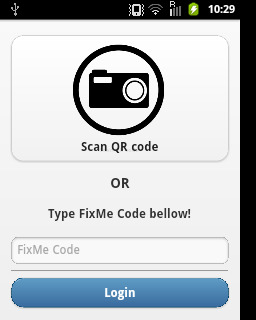
\includegraphics[scale=0.7]{login-old.png}
	\end{subfigure}
	~
	\begin{subfigure}
	\centering	
	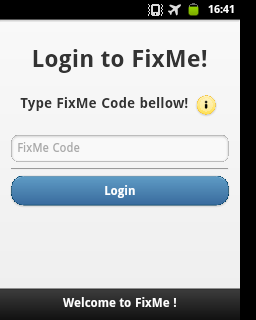
\includegraphics[scale=0.7]{l1.png}
	\end{subfigure}
	~	
	\caption{Screenshots of the old log-in screen(left) and the re-designed log-in screen(right).}	
\label{fig:login}
\end{figure}

\begin{figure}
\centering
\begin{subfigure}
	\centering	
	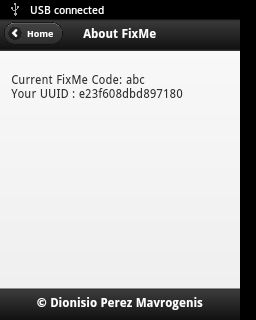
\includegraphics[scale=0.7]{help-old.png}
	\end{subfigure}
	~%spacing between figures 
	\begin{subfigure}
	\centering	
	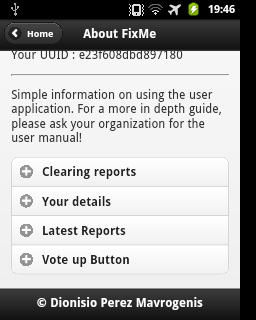
\includegraphics[scale=0.7]{help-new.png}
	\end{subfigure}
	~	
	\caption{Screenshots of the old help section(left) and the re-designed help section(right).}	
\label{fig:help}
\end{figure}

\begin{figure}
\centering
	\begin{subfigure}
	\centering	
	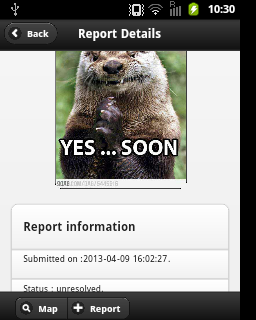
\includegraphics[scale=0.7]{report-old.png}
	\end{subfigure}
	~
	\begin{subfigure}
	\centering	
	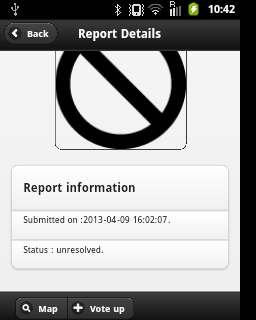
\includegraphics[scale=0.7]{report-new.png}
	\end{subfigure}
	~
	\caption{Renaming the \textit{Report} button to better convey its affordance.}	
\label{fig:repbtn}
\end{figure}

I performed several modifications to the mobile applications in order to make the application more usable. 

Help on the mobile application is now available, with confusing tasks described in a compact format under the existing \textit{Help} section, as well as displaying a helpful message on the log-in screen, as seen in figures \ref{fig:help} and \ref{fig:login}.

For making the application less confusing I simplified the log-in screen to remove QR code log-in functionality, figure \ref{fig:login}, and renamed the \textit{Report} button to \textit{Vote Up}, as seen in figure \ref{fig:repbtn}.

\paragraph{Website}
The most significant change was a re-ordering of information when displaying reports, as seen in figure \ref{fig:reportstable}.

The next most important modification I did was add feedback when managing users and when adding a new moderator. The list of moderators now gets updated dynamically when adding a new moderator and feedback is given when managing users, seen in figure \ref{fig:usrmod}.

The default displays for the \textit{Reports} and \textit{Moderators} pages became the \textit{Unresolved Reports} and \textit{View Moderators} lists, shown in \ref{fig:reportstable} and \ref{fig:usrmod} respectively.

Finally, editing of more account settings was not implemented as it was only expressed by one participant.

\begin{figure}
\centering
	\begin{subfigure}
	\centering	
	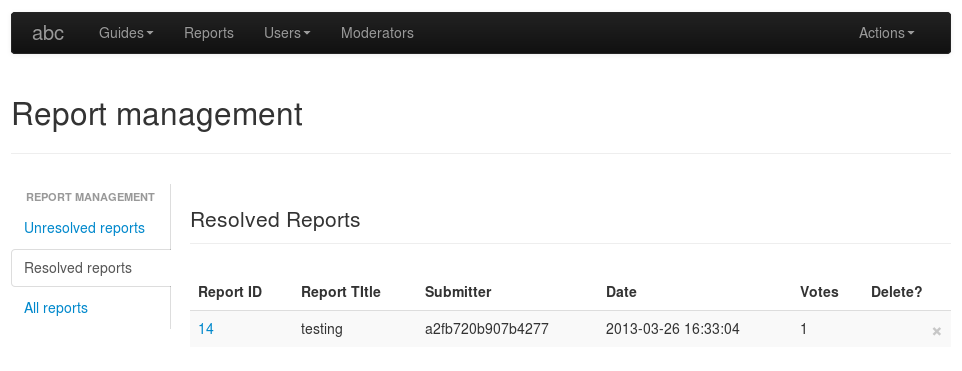
\includegraphics[scale=0.4]{resolved-old.png}
	\end{subfigure}
	~
	\begin{subfigure}
	\centering	
	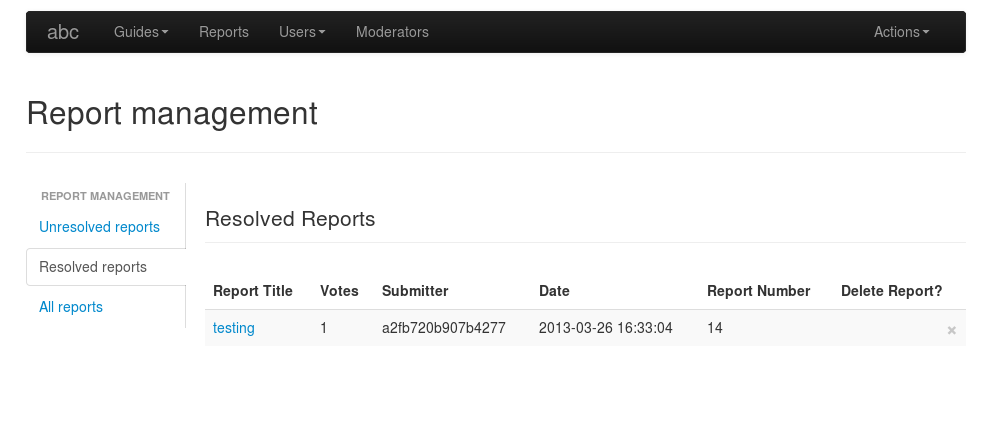
\includegraphics[scale=0.4]{order-new.png}
	\end{subfigure}
	~
	\caption{Reordering columns of the table in order to better display the useful information (old design - top, new design - bottom).}	
\label{fig:reportstable}
\end{figure}

\begin{figure}
\centering
	\begin{subfigure}
	\centering	
	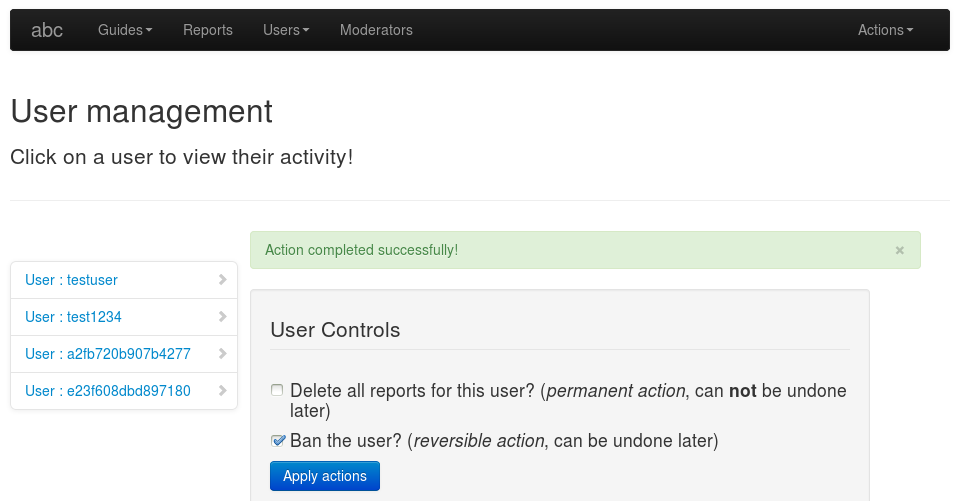
\includegraphics[scale=0.4]{usr-feedback-new.png}
	\end{subfigure}
	~
	\begin{subfigure}
	\centering	
	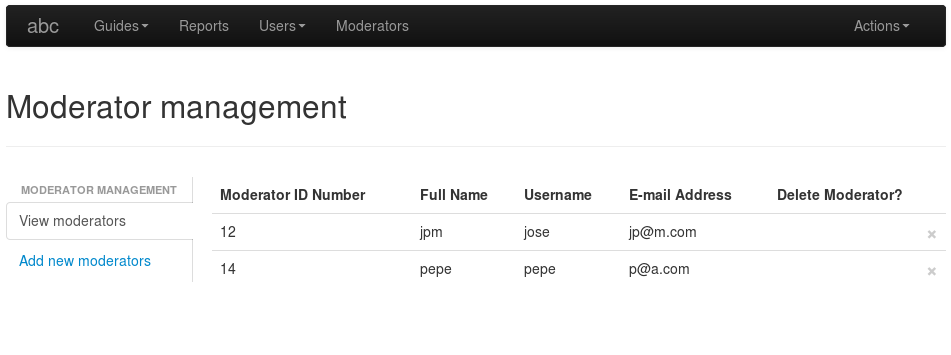
\includegraphics[scale=0.4]{mod.png}
	\end{subfigure}
	~
	\caption{Above - Feedback given when managing users ; Bottom - the dynamically updated list of moderators.}	
\label{fig:usrmod}
\end{figure}


\section{Requirements Fulfilment}
In this section I will be going through the requirements for each component and demonstrate that the current product fulfils its requirements.

Technical details on how these features are implemented are given in \ref{app:techs}.
\subsection{Mobile Applications}
After the user acceptance testing stage it is verified that non-functional requirements \texttt{1} and \texttt{2} have been met for the mobile applications. The application's size on the testing device is reported to be 2.43 megabytes, however the size of the files that I produced is only 255 kilobytes. The extra overhead is added by the Build service, something outside my control. The final size of the application is not too large\footnote{Android application supported sizes : \href{https://support.google.com/googleplay/android-developer/answer/113469}{https://support.google.com/googleplay/android-developer/answer/113469}} and it can be argued that requirement \texttt{3} is also met, since no redundant files are included in the applications.

The functional requirements of the mobile applications are reviewed bellow.

For the user mobile application, table \ref{tab:urf} contains information on the requirements fulfilment of the application. All requirements are met, further improvements could be made however.

\begin{table}
\begin{tabular}{ c | c | p{10cm}}
\textbf{Number} & \textbf{Met?} & \textbf{Comments} \\
\hline
\texttt{1} & met & none \\
\texttt{2} & met & none \\
\texttt{3} & met & none \\
\texttt{4} & met & The existence of these is verified as they are added programmatically in the mobile application and checked for empty values by the web-application. The report is rejected if a required value is empty. \\
\texttt{5 , 6} & met & Available when submitting a new report.\\
\texttt{7} & met & Mode can be switched when submitting a new report. Report details can be entered in the \textit{Settings} menu. If the mode is eponymous and the details are empty, the report is rejected.\\
\texttt{8} & met & The user can download reports of other users for a given organization by \\
\texttt{9} & met & Available through the \textit{History} screen.\\
\texttt{10} & met & none \\
\texttt{11} & met & none \\
\texttt{12}, \texttt{13} & met & Available when viewing the full details of a report.\\
\texttt{14} & met & The application queries the web-application only about unresolved reports.\\
\end{tabular}
\caption{Requirements fulfilment for the user mobile application.}
\label{tab:urf}
\end{table}

Table \ref{tab:srf} describes the requirements fulfilment status for the staff mobile application.

\begin{table}
\begin{tabular}{ c | c | p{10cm}}
\textbf{Number} & \textbf{Met?} & \textbf{Comments} \\
\hline
\texttt{1} & met & Staff members are required to login and are authenticated only if they are added via the website. \\
\texttt{2} & met & none \\
\texttt{3} & met & Available under \textit{Assigned}.\\
\texttt{4} & met & Available under \textit{Newest}. \\
\texttt{5, 6, 7} & met & Available when viewing the full details of a report.\\
\texttt{8} & met & Available under \textit{Map Overview}.\\
\end{tabular}
\caption{Requirements fulfilment for the staff mobile application.}
\label{tab:srf}
\end{table}

\subsection{Web-application}
Table \ref{tab:warf} describes the requirements fulfilment of the web-application. 

\begin{table}
\begin{tabular}{ c | c | p{10cm}}
\textbf{Number} & \textbf{Met?} & \textbf{Comments} \\
\hline
\texttt{1, 4} & met & The web-applications use PHP's native functions for content and file filtering. \\
\texttt{2} & met & none \\
\texttt{3} & met & Partially fulfilled, currently works only with the \texttt{JPEG} image format.\\
\end{tabular}
\caption{Requirements fulfilment for the staff mobile application.}
\label{tab:warf}
\end{table}


\subsection{Website}
For the website, all functional requirements have been met. Details on which security features are implemented for on website can be found in \ref{app:techs}.

Completion of the non functional requirements for the website can be seen in table \ref{tab:wsrf}. Non-functional requirement \texttt{4} is marked as partially complete because in some pages content that is not relevant to that page (mainly CSS files) is downloaded.

\begin{table}
\begin{tabular}{ c | c | p{10cm}}
\textbf{Number} & \textbf{Met?} & \textbf{Comments} \\
\hline
\texttt{1} & met & Bootstrap was designed to be responsive, as well as confirmed in testing.\\
\texttt{2, 3, 6} & met & User acceptance testing confirmed that. \\
\texttt{4} & partially met & Files that are framework specific are downloaded whether they are needed or not.\\
\texttt{5} & met & Enhanced by iterating after user acceptance testing.\\
\texttt{7} & met & Designed with HTML5 and CSS3, both with the bootstrap framework and with custom coding.\\
\end{tabular}
\caption{Non functional requirements fulfilment for the website.}
\label{tab:wsrf}
\end{table}


\chapter{Conclusion and Future Work}
\label{chap:conc}
\section{Future Work}
Future work on the framework can be dictated by two sources. Firstly, I know what needs to be improved because I have created the framework and, secondly, features could be added or improved by looking at suggestions gathered through user acceptance testing.

\subsection{Developer Insight}
Although an attempt was made to implement the following features and the software foundations exist in the source code, they were ultimately not implemented because time did not allow for the implementation and testing of these. Additionally, the extra functionality offered was not critical for making the framework work and therefore they were not given high priority.

\paragraph{\large{User and staff applications.}}
The performance of the mobile applications could be improved in a number of ways. A brief list of those is described bellow.
\begin{itemize}
\item[\textbf{Memory Management}]\hfill \\
Currently a user is a able to delete reports, however they will either delete a whole category of reports or none at all. That could change by adding a delete button to each report when listing them or when viewing their full details. Furthermore, reports are currently only removed from the phone's locally stored SQLite database, however the images that are downloaded still remain on the phone. A further improvement for better memory management would be to delete the report's image, if there is one, from the phone's memory.
\item[\textbf{Maps API}]\hfill\\
Each time the application starts, the mobile applications download the Google Maps API Javascript file. This is inconvenient because it consumes bandwidth that the users might not be willing to spend, increases the start-up time of the applications and if it fails to download it will make the applications behave unexpectedly as well as the user receiving no notification that the download has failed.

This issue exists because I have not found a way to store the API files for off-line use.

\item[\textbf{Image File Types}]\hfill \\
Currently the application does not check for the mime type of the attached image. However, as an extra measure of security the application could provide the mime type as well when an imaged be attached by the user.

To ensure secure file uploading the mime type of the image is being checked by the web application.
\end{itemize}

\paragraph{\large{Web application and website.}} The improvements that I am discussing regarding the web applications are not directly related to improvements in application performance, however I believe that these features will help the service perform better in the long term.

\begin{itemize}
\item[\textbf{Memory Management}]\hfill \\
As with the mobile applications, images are not deleted from the server when reports are removed from the database. This will have a negative impact in the storage space used by the application in the long run and it is therefore critical to remove unnecessary images in order to ensure performance.
\item[\textbf{Improved image compression}]\hfill\\
Currently the web application only supports image handling and compression of \texttt{jpeg} images. This feature is unstable and other file types are not supported, however the application would benefit by supporting handling and compression of other popular image types. PHP offers native support for compressing images that are not \texttt{jpeg}.
\item[\textbf{User limitations and statistics}]\hfill\\
Limiting the amount of disk space that a user will have available could be a good idea. Notifying users of the amount of disk space that their accounts are taking up and what space is still available would give them a strong incentive to clean up their submitted reports periodically.
\item[\textbf{Limit voting}]\hfill\\
Currently voting up of a report is not limited and the feature is prone to abuse by users attempting to attract attention to their reports.

Limiting voting to at most a vote per user per report would make the voting mechanism truly reflect the gravity of a reported issue.
\item[\textbf{Account deletion}]\hfill \\
Adding an administrative interface for deleting accounts(and related files or database entries) of organizations that registered for the FixMe service and no longer wish to use FixMe could help improve disk storage and database performance.
\item[\textbf{Security increase}]\hfill \\
The security of the framework could be hardened by security additions such as email activation of the account registered or chaptcha images in order to avoid brute-forcing of accounts or mass registrations of new accounts, just to name a few.
\end{itemize}

\subsection{User feedback}
Future work described here is derived by analysing user feedback that was obtained through user acceptance testing. The work described here is what was not implemented during iteration over the design and functionality of the applications, mainly because of time restrictions. The views described here do not necessarily represent all participants collectively.

\begin{itemize}
\item[\textbf{Application installation}]\hfill \\
A view that was collectively expressed by all participants taking place in testing the mobile applications was that they would prefer for the application to exist in their platform's app-store.

It is sensible that users prefer an automated method of installing applications on their phone from the official app-store of their respective platforms over the current manual procedure. Furthermore users are more likely to trust and install an application from the app-store rather than some random website they've never heard of before.

This feature was not implemented because maintenance and distribution of the application over multiple platforms and app-stores was beyond the scope of this project.

\item[\textbf{E-mail activation}]\hfill\\
A large portion of the users that participated in testing the website were observed to look for an account activation email in their inbox.

Although the software foundations exist for such a feature to exist, the feature was never implemented because emphasis was placed on more important functionality. However this feature is useful to have as an additional security measure.
\item[\textbf{Removal of functionality}]\hfill \\
Certain participants expressed that having a \textit{Favourites} section and functionality in the application was useless. The functionality was not removed as it was not universally declared useless, however, this provides a good point for further investigation.
\item[\textbf{Application appearance}]\hfill \\
The mobile applications and website could have more colours or icons.

Graphic design and appearance is beyond the scope of this project and as a result this concern was overlooked.
\end{itemize}

\subsection{Improved user testing}
Even though this is not directly related with further developing the applications, I believe that revisiting the user acceptance testing process once more would yield positive results. 

Even though user testing was performed on the components in order to refine the functionality and appearance of the applications, I feel that the user testing that I performed was not rigorous or realistic enough.

The demographic of people that took part in the user testing of my applications were between 19 and 23 years old. Additionally all participants were familiar with smart-phones and browsing the web on a daily basis. In addition to the participants being very comfortable with technology, the number of participants was small and none of them fit entirely the actual target demographic, although their feedback was critical in improving the application.

For obtaining realistic feedback the participants that should be tested should be of varying ages (roughly between 18 and 55 years of age) in order to get feedback from users that are not extremely familiar with technology and some of them would have to own or be in charge of maintaining or managing an organization, in order to get feedback or ideas for features from people who perform the task that this framework is to assist.

Furthermore, in order to get better functional and non-functional requirements users belonging in the aforementioned demographic should be consulted and allowed to express their needs and expectations from such a framework. 

Finally, field testing of the application should be mote intense and perhaps in a realistic environment in order to evaluate its true performance.

\section{Conclusion}
Looking back on the project and its development I can say that it went smoothly overall, deadlines were met and the issues that were critical to address, allowing users of the facilities of an organization to notify the organization about breakages they encounter, have been addressed.

Even though the deadlines were met and the final products were delivered, certain decisions could have been better.

The agile development methodology of the deliverables and the planning, although it worked and was adequate, could be improved. A better estimation of the threats to the time schedule would have been more helpful, since January was almost a dead period due to exams. Furthermore the user acceptance testing could have run on a tighter schedule, instead of trying to figure the most convenient slot for the participants. Thankfully, as shown in \ref{fig:charts} these delays were taken into account and the planning was revised in order to accommodate the changes.

Another issue that I feel was not carried out thoroughly was user acceptance and field testing. I feel that the amount of testing that was performed could be increased, yielding better answers to the question of how the applications could be improved. User acceptance and field testing were impacted by the availability of participants and time shortage for testing all of them thoroughly.

Finally,I feel that, although the task was well defined and completed, the scope of the project - producing both mobile and web applications - was very large. I feel that with a narrower scope, either mobile applications or web-applications, the development would have been more focused, more issues would have been addressed and the final deliverables could have been further optimised. Having said that, I feel that the final system works well, the delivered code has got quality (something that I cared for from the very beginning of the project) that is verifiable and the issues that have not been addressed have got no considerable impact on the usefulness of the framework.

\bibliography{bibl}

\appendix

\chapter{Requirements Documents}
\label{chap:reqcdocs}
\section{Mobile Applications }
\subsection{User Applications Functional Requirements}
\begin{enumerate}
\item Allow the user to select a FixMe account for submitting reports.
\item Allow the user to switch from one Fixme account to another.
\item Allow the user to submit a new report.
\item Each report \textbf{must} have a 
\begin{inparaenum}[\itshape a\upshape)]
\item report title;
\item report description;
\item a value for the latitude of the position of the report;
\item a value for the longitude of the position of the report;
\item a unique identifier indicating the device of origin;
\end{inparaenum}
\item Allow the user to optionally refine their position on the map.
\item Allow the user to optionally attach a new photograph with each report.
\item Allow the user to submit anonymous or eponymous reports.
\item Allow the user to view reports other users have submitted.
\item Allow the user to view reports they have submitted.
\item Allow the user to view full details on a report.
\item Allow the user to mark or un-mark a report as favourite.
\item Allow a user to vote up a report.
\item Allow a user to view a report's location on the map.
\item Transfer minimal amounts of network traffic.
\end{enumerate}

\subsection{Staff Application Functional Requirements}
Staff members : 
\begin{enumerate}
\item \textbf{must} authenticate themselves in order to use the application with a given FixMe account.
\item must be able to switch to a different FixMe account.
\item must be able to see the reports assigned to them.
\item must be able to see the reports of unresolved issues.
\item must be able to mark an issue as resolved.
\item must be able to view full details of a report.
\item must be able to view a report's location on the map.
\item must be able to visualize their location and all reports on a map.
\end{enumerate}

\subsection{Mobile Application Non-functional Requirements}
The non-functional requirements are common to both mobile applications and therefore are considered in a separate section
\begin{enumerate}
\item Have a clean, intuitive and non-confusing layout.
\item Have no deep or hidden sub-menus.
\item The application should be as lightweight as possible.
\end{enumerate}

\section{Web Application Requirements}
\subsection{Functional Requirements}
The application : 
\begin{enumerate}
\item should properly filter all incoming content.
\item must ensure that all incoming reports meet the minimum criteria before they are stored into the database.
\item should compress content whenever possible.
\item should handle file uploading in a safe and consistent manner.
\end{enumerate}

\section{Website Requirements}
\subsection{Functional Requirements}
The website :
\begin{enumerate}
\item \textbf{must} filter all incoming content.
\item \textbf{must} ensure that only actions of legitimate users are carried out.
\item must allow registration and member log-in.
\item must allow the user to view or delete reports submitted to them.
\item must allow the user to add or remove a moderator.
\item must allow the user to change the status of a report and/or assign it to a moderator.
\item must allow a user to ban or unban a mobile application users from submitting reports
\end{enumerate}

\subsection{Non-functional Requirements}
The website should :
\begin{enumerate}
\item be responsive.
\item have a clean, intuitive, non-confusing controls and layout.
\item have no deep or hidden sub-menus.
\item be as lightweight as possible.
\item provide appropriate feedback when actions are carried out.
\item ensure that information is found easily.
\item comply with the newest standards for web design.
\end{enumerate}


\chapter{Use Cases}
In this appendix I will be presenting the use case scenarios and use case diagrams that I produced in order to create the user requirements and verify those.
\section{Use Case Scenarios}
\textit{Administrator} represent staff members that operate the website, \textit{Staff} represents staff members that use the staff mobile application and \textit{Client} represents users of the mobile application.

\begin{enumerate}
\item Facility owner wants to deploy fixMe to their facility, process for achieving it. 
\item Facility owner wants to let his clients know of the system. 
\item Staff wants to add or remove an Administrator. 
\item Client wants to install the application. 
\item Client wants to connect application with said facility. 
\item Client wants to submit report. 
\item Client wants to browse recent reports. 
\item Client wants to view report info. 
\item Client wants to see reports on the map. 
\item Client wants to up-vote on a reported issue.
\item A client pulls the list of latest reports. 
\item Administrator wants to review a report and change its status.
\item Administrator wants to block a user of the application. 
\item Staff wants to view their assigned reports.
\item Staff toggles report status.
\end{enumerate}


\section{User case diagrams}
\begin{figure}[h]
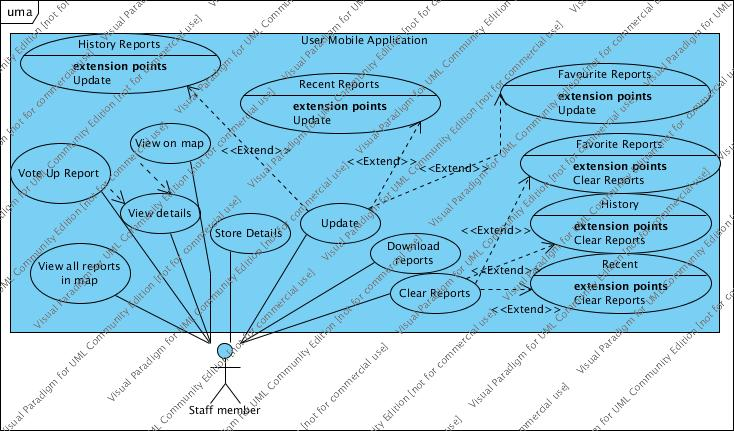
\includegraphics[scale=0.6]{uml/uma.jpg}
\caption{Use case diagram for the user mobile application.}
\end{figure}

\begin{figure}[h]
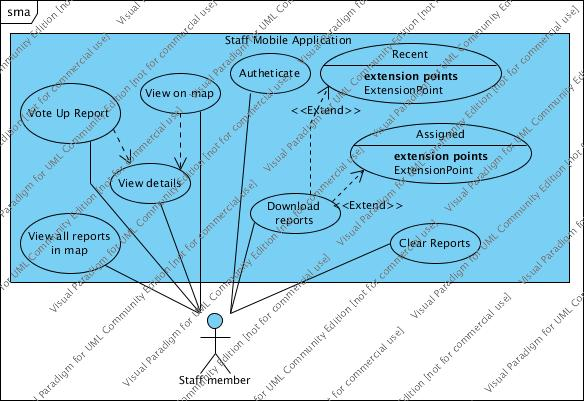
\includegraphics[scale=0.7]{uml/sma.jpg}
\caption{Use case diagram for the staff mobile application.}
\end{figure}

\begin{figure}[h]
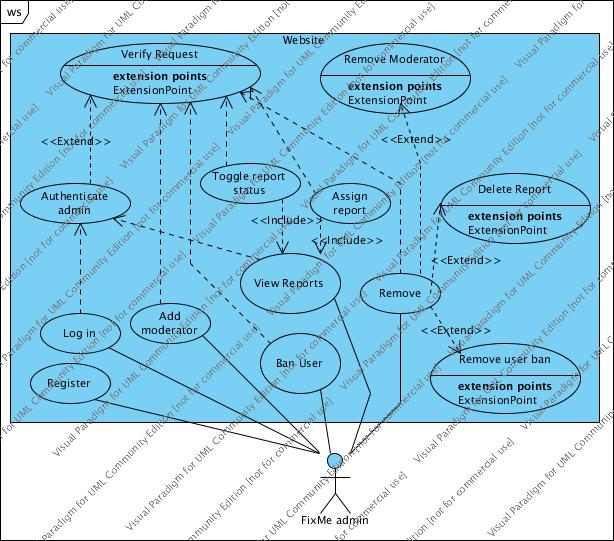
\includegraphics[scale=0.7]{uml/ws.jpg}
\caption{Use case diagram for the website.}
\end{figure}

\begin{figure}[h]
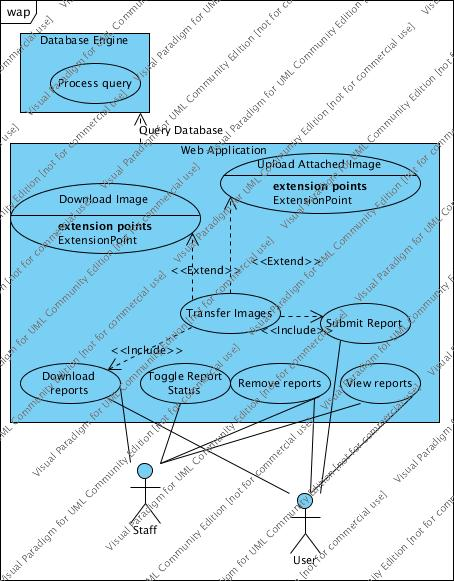
\includegraphics[scale=0.8]{uml/wap.jpg}
\caption{Use case diagram for the web application.}
\end{figure}


\chapter{Repositories and Tools Used}
\label{chap:tools}

\section{Tools and Libraries}
\subsection{External Libraries}
\label{sec:extlib}
This section will provide links to the external libraries used. Information on obtaining, installing and using the library are on those websites.

\begin{itemize}
\item[\textbf{jQuery Mobile}] \href{http://jquerymobile.com/}{http://jquerymobile.com/}
\item[\textbf{Twig}] \href{http://twig.sensiolabs.org/}{http://twig.sensiolabs.org/}
\item[\textbf{jQuery}] \href{http://jquery.com/}{http://jquery.com/}
\item[\textbf{Maps API}] \href{https://developers.google.com/maps/documentation/javascript/tutorial}{https://developers.google.com/maps/documentation/javascript/tutorial}
\item[\textbf{Bootstrap}] \href{http://twitter.github.com/bootstrap/}{http://twitter.github.com/bootstrap/}
\item[\textbf{MetroStation Icons}] \href{http://yankoa.deviantart.com/art/MetroStation-183210118}{http://yankoa.deviantart.com/art/MetroStation-183210118}
\item[\textbf{JSON2}] \href{https://github.com/douglascrockford/JSON-js/blob/master/README}{https://github.com/douglascrockford/JSON-js/blob/master/README}
\end{itemize}

\subsection{Tools Used}
\label{sec:tools}
\begin{itemize}
\item[\textbf{Trello}]\href{https://trello.com/}{https://trello.com/}
\item[\textbf{GanttProject}] \href{http://www.ganttproject.biz/}{http://www.ganttproject.biz/}
\item[\textbf{Github}]\href{https://github.com}{https://github.com}
\item[\textbf{Google Closure}]\href{https://developers.google.com/closure/}{https://developers.google.com/closure/}
\item[\textbf{JSHint}]\href{http://jshint.com/}{http://jshint.com/}
\item[\textbf{PhoneGap Build}]\href{https://build.phonegap.com}{https://build.phonegap.com}
\item[\textbf{Jetbrains WebStorm}]\href{http://www.jetbrains.com/webstorm/}{http://www.jetbrains.com/webstorm/}
\item[\textbf{Eclipse}]\href{http://www.eclipse.org/}{http://www.eclipse.org/}
\item[\textbf{WireframeSketcher}]\href{http://wireframesketcher.com/}{http://wireframesketcher.com/}
\item[\textbf{xdebug}]\href{http://xdebug.org/}{http://xdebug.org/}
\end{itemize}

\section{Github Repositories}
\label{sec:repos}
These are links to the github repositories for my third year project. 
\begin{itemize}
\item[\textbf{FixMe user application}] \href{https://github.com/dperezmavro/Andron}{https://github.com/dperezmavro/Andron}
\item[\textbf{FixMe staff application}] \href{https://github.com/dperezmavro/MAndron}{https://github.com/dperezmavro/MAndron}
\item[\textbf{FixMe web-applications}] \href{https://github.com/dperezmavro/Andron-server}{https://github.com/dperezmavro/Andron-server}
\item[\textbf{Project Documentation}] \href{https://github.com/dperezmavro/3ypdoc}{https://github.com/dperezmavro/3ypdoc}
\end{itemize}

\textbf{Note : }The web-application repository, containing both the web application and the website code, is private because it contains files with sensitive information. These files are included in the CD however.

\chapter{Project Planning}
\section{Gantt Charts}

In this section Gantt charts showing how work was planned and was actually carried out are shown.

The colours in the Gantt charts indicate :

\textcolor{purple}{Purple } : Testing and iteration. This includes module, integration, system, user and acceptance testing and the iteration over those.

\colorbox{black}{\textcolor{yellow}{Yellow }} : This includes writing the deliverables (progress or project report).

\textcolor{blue}{Blue } : This indicates software development.

\begin{landscape}
\begin{figure}
\centering
	\begin{subfigure}
	\centering	
	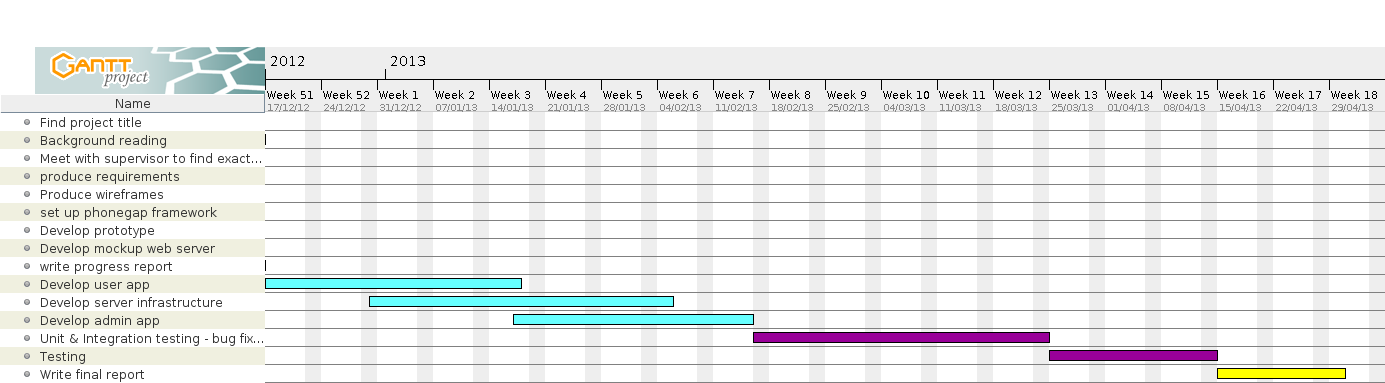
\includegraphics[scale=0.5]{rem.png}
	\caption{Initial estimate and alocation of tasks after completing prototype.}
	\label{fig:ganorig}
	\end{subfigure}
	~
	\begin{subfigure}
	\centering	
	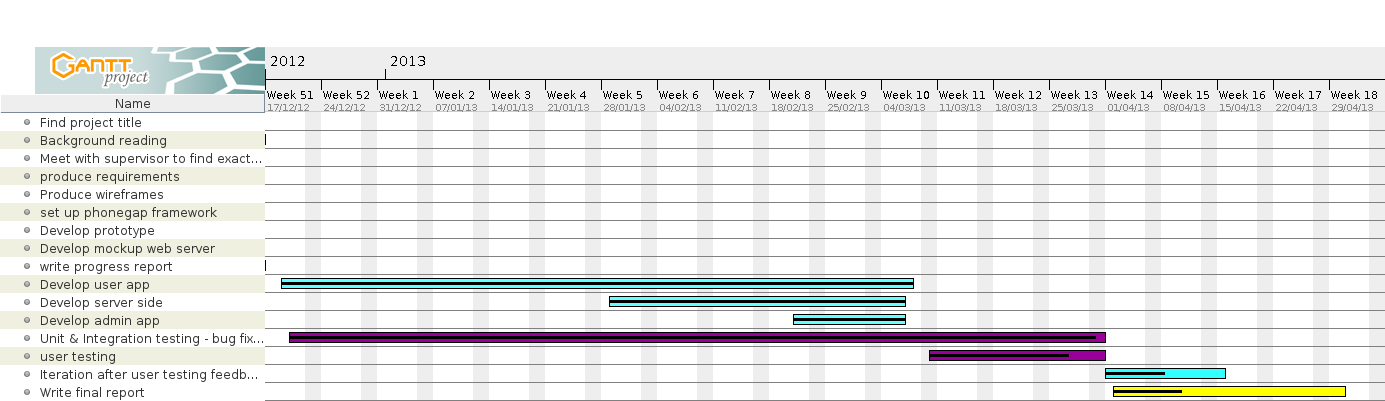
\includegraphics[scale=0.5]{final.png}
	\caption{Schedule and task completion as it was finally scheduled.}
	\label{fig:ganfin}
	\end{subfigure}
	~%spacing between figures 	
\label{fig:charts}
\end{figure}
\end{landscape}

\chapter{Technical Specification}
\label{app:techs}
This section described the technical details of how the various features of the components of FixMe are implemented.
\section{Mobile Applications}
\textbf{Implementation Language : } HTML5, CSS3 and Javascript.

\textbf{Data transfer : } Data will be transferred in JSON format and using asynchronous AJAX calls, in order to avoid blocking (except for the login screen). Queries regarding report status updates will be made for unresolved reports only, in order to minimise the amount of data sent and received.

\textbf{Data Storage : } Data will be stored on the mobile device by using an SQLite database on the phones local-storage. User details for eponymous posting will be saved in a table name \texttt{user\_details} and reports will be stored in tables \textbf{fav\_reports}, \textbf{recent\_reports} and  \textbf{history\_reports} for the user application and \textbf{recent\_reports} and \textbf{watchlist\_reports} for the staff application.

Images downloaded with the reports will be stored on the phone's file storage.

The staff mobile application will also be making use of a randomly generated token on a per-login for verifying the authenticity of the request, in order to avoid people abusing the service.

In order to save space, the ability to clear the SQLite databases should be provided.

\section{Database}
The database will store all information required to make the framework work.
\textbf{Implementation Language : } MySQL

\textbf{Database Schema : }

\begin{table}[ht]
\begin{tabular}[ht]{p{5cm} | p{8cm} }
\texttt{andron\_authorities\_table} & holds the registered FixMe users. \\ 
\hline
\texttt{aa\_reports} & holds all the reports submitted.\\
\hline
\texttt{aa\_mods} & A table holding information on the staff members allows to used the FixMe Staff application. \\
\hline
\texttt{assignments} &  A table that holds reports assigned to staff members. \\
\hline
\texttt{aa\_balist} & A table that holds information on banned users. \\
\end{tabular}
\caption{Overview of the tables of the FixMe framework.}
\end{table}

\section{Web application}
\textbf{Implementation Language : } PHP.
The web application will be responsible for storing and retrieving reports from the MySQL database, as well as handling file uploads.

\textbf{Security features : }
\begin{itemize}
\item Content will be filtered for guarding against XSS with PHP's \texttt{htmlentities} function before being stored in the database.
\item Prepared statements will be used to access the database in order to avoid SQL injections.
\item Directory listings will be prevented by using the appropriate directives in \texttt{.htaccess} files.
\item File uploading functionality will rename the file using a random string and will also append an extension to the final file name.
\end{itemize}

\textbf{Image compression : } The application will compress \textbf{JPEG} images using PHP's \texttt{imagecreatefromjpeg} and \texttt{imagejpeg} functions in order to minimise disk space consumption.

\section{Website}
\textbf{Implementation Language : } PHP, HTML5, Javascript and CSS3. Additionally, Bootstrap will be used to present the templates that are rendered by Twig.

Javascript and AJAX requests will be used to dynamically update the website and carry out actions, in order to avoid having to refresh the page to view changes and make the website more user friendly.

\textbf{Security features : }
\begin{itemize}
\item Random tokens are used to prevent CSRF.
\item Passwords stored in the database will be hashed.
\item Accessing the database will happen only through prepared statemetns.
\item \texttt{htmlentities} will be used to protect against XSS.
\end{itemize}


\chapter{Source Code Listing}
In this appendix only the database MySQL file is being listed. Other source code files are too big to be listed, however they can be found on the CD provided together with this document.

\section{The Database}
This is the MySQL database that supports the FixMe framework. The file can be found in \texttt{server/fixme.sql} on the accompanying CD.
\lstinputlisting[language=SQL,
	caption=MySQL database of the FixMe framework.,
	breaklines=true,
	numbers=left,
	numberstyle=\tiny,
	label=mysqldblst]{./files/fixme.sql}


\chapter{User Testing Guides}
The testing guide document is not included in this document because it is very lengthy, as it comprises of tests for all of the components. 

The testing guide that was provided to the participants of the user testing can be downloaded from Dropbox, by clicking on the URL : \\ \href{http://dl.dropbox.com/u/23023752/usertesting.pdf}{http://dl.dropbox.com/u/23023752/usertesting.pdf}.
\label{app:testing}


\chapter{CD Contents}
List of CD contents.
\begin{table}[th]
\begin{tabular}{c | p{12cm}}
\large{\textbf{Folder}} & \large{\textbf{Contents}} \\
\hline
\textbf{userapp} & Folder containing files for the user mobile application. for details see \ref{sec:userdir}.\\
\hline
\textbf{staffapp} & Folder containing the files for the staff mobile application. For details please see \ref{sec:staffdir}. \\
\hline
\textbf{server} & Folder containing the files for the website and web-application. For details see \ref{sec:srvdir}.\\
\hline
\textbf{doc} & Folder containing documentation files and deliverables. For details see \ref{sec:docdir}.\\
\hline
\end{tabular}
\end{table}

\section{userapp}
\label{sec:userdir}

\section{staffapp}
\label{sec:staffdir}

\section{server}
\label{sec:srvdir}

\section{doc}
\label{sec:docdir}

\end{document}
